%%
%% This is file `sample-manuscript.tex',
%% generated with the docstrip utility.
%%
%% The original source files were:
%%
%% samples.dtx  (with options: `manuscript')
%% 
%% IMPORTANT NOTICE:
%% 
%% For the copyright see the source file.
%% 
%% Any modified versions of this file must be renamed
%% with new filenames distinct from sample-manuscript.tex.
%% 
%% For distribution of the original source see the terms
%% for copying and modification in the file samples.dtx.
%% 
%% This generated file may be distributed as long as the
%% original source files, as listed above, are part of the
%% same distribution. (The sources need not necessarily be
%% in the same archive or directory.)
%%
%% Commands for TeXCount
%TC:macro \cite [option:text,text]
%TC:macro \citep [option:text,text]
%TC:macro \citet [option:text,text]
%TC:envir table 0 1
%TC:envir table* 0 1
%TC:envir tabular [ignore] word
%TC:envir displaymath 0 word
%TC:envir math 0 word
%TC:envir comment 0 0
%%
%%
%% The first command in your LaTeX source must be the \documentclass command.
%%%% Small single column format, used for CIE, CSUR, DTRAP, JACM, JDIQ, JEA, JERIC, JETC, PACMCGIT, TAAS, TACCESS, TACO, TALG, TALLIP (formerly TALIP), TCPS, TDSCI, TEAC, TECS, TELO, THRI, TIIS, TIOT, TISSEC, TIST, TKDD, TMIS, TOCE, TOCHI, TOCL, TOCS, TOCT, TODAES, TODS, TOIS, TOIT, TOMACS, TOMM (formerly TOMCCAP), TOMPECS, TOMS, TOPC, TOPLAS, TOPS, TOS, TOSEM, TOSN, TQC, TRETS, TSAS, TSC, TSLP, TWEB.
% \documentclass[acmsmall]{acmart}

%%%% Large single column format, used for IMWUT, JOCCH, PACMPL, POMACS, TAP, PACMHCI
% \documentclass[acmlarge,screen]{acmart}

%%%% Large double column format, used for TOG
% \documentclass[acmtog, authorversion]{acmart}

%%%% Generic manuscript mode, required for submission
%%%% and peer review
\documentclass[manuscript,screen,review]{acmart}
%% Fonts used in the template cannot be substituted; margin 
%% adjustments are not allowed.
%%
%% \BibTeX command to typeset BibTeX logo in the docs
\AtBeginDocument{%
  \providecommand\BibTeX{{%
    \normalfont B\kern-0.5em{\scshape i\kern-0.25em b}\kern-0.8em\TeX}}}

%% Rights management information.  This information is sent to you
%% when you complete the rights form.  These commands have SAMPLE
%% values in them; it is your responsibility as an author to replace
%% the commands and values with those provided to you when you
%% complete the rights form.
\setcopyright{acmcopyright}
\copyrightyear{2018}
\acmYear{2018}
\acmDOI{XXXXXXX.XXXXXXX}

%% These commands are for a PROCEEDINGS abstract or paper.
\acmConference[Conference acronym 'XX]{Make sure to enter the correct
  conference title from your rights confirmation emai}{June 03--05,
  2018}{Woodstock, NY}
%
%  Uncomment \acmBooktitle if th title of the proceedings is different
%  from ``Proceedings of ...''!
%
\acmBooktitle{Woodstock '18: ACM Symposium on Neural Gaze Detection,
 June 03--05, 2018, Woodstock, NY} 
\acmPrice{15.00}
\acmISBN{978-1-4503-XXXX-X/18/06}


%%
%% Submission ID.
%% Use this when submitting an article to a sponsored event. You'll
%% receive a unique submission ID from the organizers
%% of the event, and this ID should be used as the parameter to this command.
%%\acmSubmissionID{123-A56-BU3}

%%
%% For managing citations, it is recommended to use bibliography
%% files in BibTeX format.
%%
%% You can then either use BibTeX with the ACM-Reference-Format style,
%% or BibLaTeX with the acmnumeric or acmauthoryear sytles, that include
%% support for advanced citation of software artefact from the
%% biblatex-software package, also separately available on CTAN.
%%
%% Look at the sample-*-biblatex.tex files for templates showcasing
%% the biblatex styles.
%%

%%
%% The majority of ACM publications use numbered citations and
%% references.  The command \citestyle{authoryear} switches to the
%% "author year" style.
%%
%% If you are preparing content for an event
%% sponsored by ACM SIGGRAPH, you must use the "author year" style of
%% citations and references.
%% Uncommenting
%% the next command will enable that style.
%%\citestyle{acmauthoryear}

%%
%% end of the preamble, start of the body of the document source.
\begin{document}

\title{Task 4  Numerical Methods}
\author{Carl-Emil Rohde \\ kvb125@alumni.ku.dk}
\date{September 2023}

\maketitle

\section*{Problem 1}
 \begin{center}
    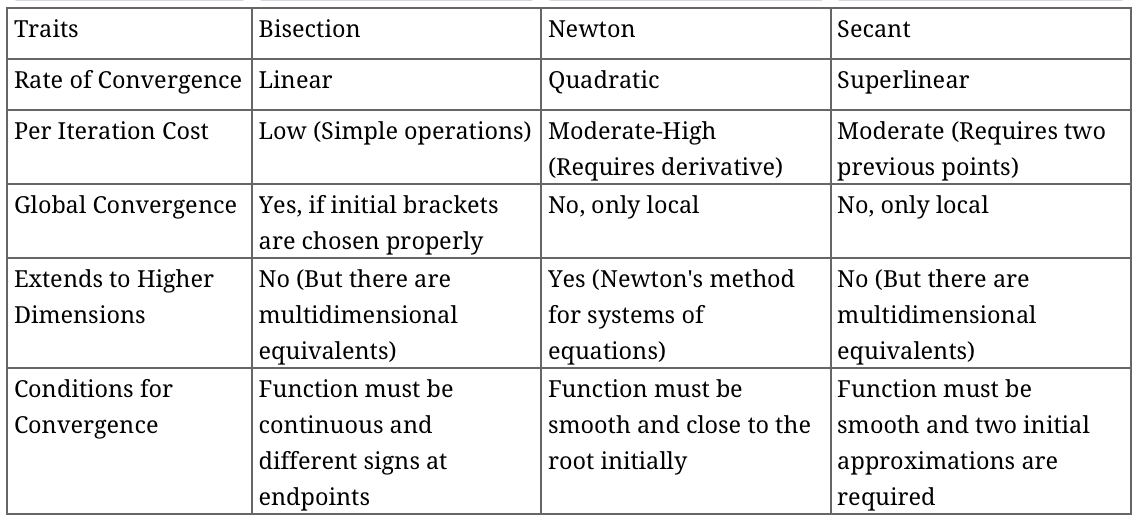
\includegraphics[scale=0.41]{Screenshot 2023-09-30 at 13.32.35.png}
\end{center}

\section*{Problem 2}
\subsection*{3.1.2}
\textbf{a)}
According to the content on page 78 , the width of the interval at the $n$'th step is given by:
$$
b_n-a_n=2^{-n}\left(b_0-a_0\right)
$$
For the initial interval $[1.5,3.5], b_0=3.5$ and $a_0=1.5$. So, $b_0-a_0=3.5-1.5=2$.
Therefore, the width of the interval at the $n$'th step would be:
$$
b_n-a_n=2^{-n} \times 2=2^{-n+1}
$$
\textbf{b)}
The maximum distance between the root $r$ and the midpoint $c_n$ of the interval $\left[a_n, b_n\right]$ is given by:
$$
\left|r-c_n\right| \leq \frac{1}{2}\left(b_n-a_n\right)
$$
Using the expression for $b_n-a_n$ I derived before, this inequality becomes:
$$
\left|r-c_n\right| \leq \frac{1}{2} \times 2^{-n+1}=2^{-n}
$$
Thus, the maximum distance possible between the root $r$ and the midpoint of the interval at the $n$'th step is $2^{-n}$.

\subsection*{3.1.9}
For the case $\left[a_0, b_0\right]=[0,1]$, the root $r$ in binary representation can be expressed as $r=$ $0 . d_1 d_2 d_3 \ldots$
In decimal form, $r=\sum_{n=1}^{\infty} \frac{d_n}{2^n}$.
For a general interval $\left[a_0, b_0\right]$, the root $r$ is:
$$
r=a_0+\left(b_0-a_0\right) \sum_{i=1}^{\infty} \frac{d_i}{2^i}
$$
Here $d_n=0$ if the interval at the $n$-th step is the left half of the previous interval, and $d_n=$ 1 otherwise.

\subsection*{3.2.9}
To solve for $x_2$ using Newton's method, I first need to find the derivative $f^{\prime}(x)$ of $f(x)=x^3-2$. The derivative is $f^{\prime}(x)=3 x^2$.
Newton's method uses the formula:
$$
x_{n+1}=x_n-\frac{f\left(x_n\right)}{f^{\prime}\left(x_n\right)}
$$
Starting with $x_0=1$, let's find $x_1$ and then $x_2$.
To find $x_1$ :
$$
\begin{gathered}
x_1=x_0-\frac{f\left(x_0\right)}{f^{\prime}\left(x_0\right)} \\
x_1=1-\frac{(1)^3-2}{3(1)^2} \\
x_1=1-\frac{-1}{3} \\
x_1=1+\frac{1}{3} \\
x_1=\frac{4}{3}
\end{gathered}
$$
To find $x_2$ :
\begin{align*}
x_2 &= x_1-\frac{f\left(x_1\right)}{f^{\prime}\left(x_1\right)} &
x_2 &= \frac{4}{3}-\frac{\left(\frac{4}{3}\right)^3-2}{3\left(\frac{4}{3}\right)^2} \\
x_2 &= \frac{4}{3}-\frac{\frac{64}{27}-\frac{54}{27}}{3 \cdot \frac{16}{9}} &
x_2 &= \frac{4}{3}-\frac{\frac{10}{27}}{\frac{48}{27}} \\
x_2 &= \frac{4}{3}-\frac{10}{48} &
x_2 &= \frac{4}{3}-\frac{5}{24} \\
x_2 &= \frac{96}{72}-\frac{15}{72} &
x_2 &= \frac{81}{72} \\
x_2 &= \frac{9}{8}
\end{align*}

Thus, $x_2=\frac{9}{8}$.

\subsection*{3.3.4}
The formula for the secant method is given by:
$$
x_{n+1}=x_n-f\left(x_n\right)\left[\frac{x_n-x_{n-1}}{f\left(x_n\right)-f\left(x_{n-1}\right)}\right]
$$
To find $x_2$, I'll use $x_0=0$ and $x_1=1$ as $x_{n-1}$ and $x_n$ respectively in the formula.
Firstly, I  will evaluate $f\left(x_0\right)$ and $f\left(x_1\right)$ :
$$
\begin{aligned}
& f\left(x_0\right)=f(0)=0^2-2=-2 \\
& f\left(x_1\right)=f(1)=1^2-2=-1
\end{aligned}
$$
Now, I substitute these into the formula to find $x_2$ :
$$
\begin{gathered}
x_2=x_1-f\left(x_1\right)\left[\frac{x_1-x_0}{f\left(x_1\right)-f\left(x_0\right)}\right] \\
x_2=1-(-1)\left[\frac{1-0}{-1-(-2)}\right] \\
x_2=1+\frac{1}{1} \\
x_2=1+1 \\
x_2=2
\end{gathered}
$$
So, $x_2$ is 2 when we apply the secant method to the function $f(x)=x^2-2$ with $x_0=0$ and $x_1=1$.

\subsection*{3.5.1}
I want to use Horner's Algorithm to evaluate $p(4)$, where the polynomial $p(z)$ is given by
$$
p(z)=3 z^5-7 z^4-5 z^3+z^2-8 z+2
$$
We have the coefficients $a_0, a_1, \ldots, a_5$ of $p(z)$ :
$$
a_5=3, \quad a_4=-7, \quad a_3=-5, \quad a_2=1, \quad a_1=-8, \quad a_0=2
$$
I'll set $z_0=4$ and use Horner's algorithm to find $p(4)$.
I arrange the calculation according to the tabular method suggested on page 112:
\\
\\
\begin{tabular}{r|rrrrrr}
4 & 3 & -7 & -5 & 1 & -8 & 2 \\
& & 12 & 20 & 60 & 220 & 848 \\
\hline & 3 & 5 & 15 & 61 & 212 & 850
\end{tabular}
\\
\\
Here's how the calculations were done step-by-step:
$$
\begin{aligned}
& b_4=a_5=3 \\
& b_3=a_4+z_0 b_4=-7+4 \times 3=5 \\
& b_2=a_3+z_0 b_3=-5+4 \times 5=15 \\
& b_1=a_2+z_0 b_2=1+4 \times 15=61 \\
& b_0=a_1+z_0 b_1=-8+4 \times 61=212 \\
& p(4)=a_0+z_0 b_0=2+4 \times 212=850 \\
& \text { So, } p(4)=850
\end{aligned}
$$
Additionally, the resulting polynomial $q(z)$ (of degree one less than $p(z)$ ) is:
$$
q(z)=3 z^4+5 z^3+15 z^2+61 z+212
$$
Thus, can also represent $p(z)$ as:
$$
p(z)=(z-4) q(z)+p(4)=(z-4)\left(3 z^4+5 z^3+15 z^2+61 z+212\right)+850
$$

\section*{Problem 3}
The goal is to find an approximation to $\sqrt{7}$ with an accuracy of $10^{-7}$ using the secant method. I will model this as a root-finding problem.
\\
The secant method is an iterative numerical method used for finding roots of a function $f(x)$. Given two initial guesses $x_0$ and $x_1$, the secant method iteratively refines these guesses using the formula:
$$
x_{n+1}=x_n-\frac{f\left(x_n\right) \cdot\left(x_n-x_{n-1}\right)}{f\left(x_n\right)-f\left(x_{n-1}\right)}
$$
The method stops when the absolute value of $f(x)$ is less than a given tolerance $\epsilon$ or the relative error between successive approximations is less than or equal to $\epsilon$.
\\
We start with initial guesses close to $\sqrt{7}$ :
\\
- $x_0=2.5$ (a bit less than $\sqrt{7}$ )
\\
- $x_1=3.0$ (a bit more than $\sqrt{7}$ )
\\
The tolerance level $\epsilon$ is set to $10^{-7}$ as per the problem statement.
\\
The secant method was implemented to find the root of $f(x)=$ $x^2-7$, using the initial guesses and tolerance level mentioned above.
\\
\\
After 4 iterations, the method converged to an approximate root of 2.64575131094764, meeting the specified accuracy level of $10^{-7}$.

\section*{Problem 4}
To find the surface area $S$ of a cone, the formula is:
$$
S=\pi r^2+\pi r l
$$
Where $r$ is the radius and $l$ is the slant height. The slant height $l$ can be related to the radius $r$ and height $h$ through the Pythagorean theorem:
$$
l=\sqrt{r^2+h^2}
$$
Given that $S=1200 \mathrm{~m}^2$ and $h=20 \mathrm{~m}$, I can plug these into the formulas:
$$
1200=\pi r^2+\pi r \sqrt{r^2+400}
$$
Now, I rewrite this equation as a root-finding problem $f(x)=0$ :
$$
f(r)=\pi r^2+\pi r \sqrt{r^2+400}-1200=0
$$
To solve the problem using the Secant method, I start with two initial guesses $x_0$ and $x_1$ for the radius $r$, and then iterate using the formula:
$$
x_{n+1}=x_n-f\left(x_n\right) \frac{x_n-x_{n-1}}{f\left(x_n\right)-f\left(x_{n-1}\right)}
$$
For the function $f(r)=\pi r^2+\pi r \sqrt{r^2+400}-1200$, I have implemented the Secant method in Python. When i run the code, i get that the approximate radius is 11,19, and the number of iterations to achieve the desired accuracy is 5. 

Mathematically, super-linear convergence is often characterized as follows:
$$
\lim _{n \rightarrow \infty} \frac{\epsilon_{n+1}}{\epsilon_n^p}=C
$$
Here $C$ is a constant and $p>1$, but $p \neq 2$.
To make a convergence plot, we want to track the absolute error $\left|\epsilon_n\right|=\left|x_n-x_{\text {root }}\right|$ at each iteration $n$. 
\\
\\
I have implemented some Python code that does this, and produce the following plot:
\\
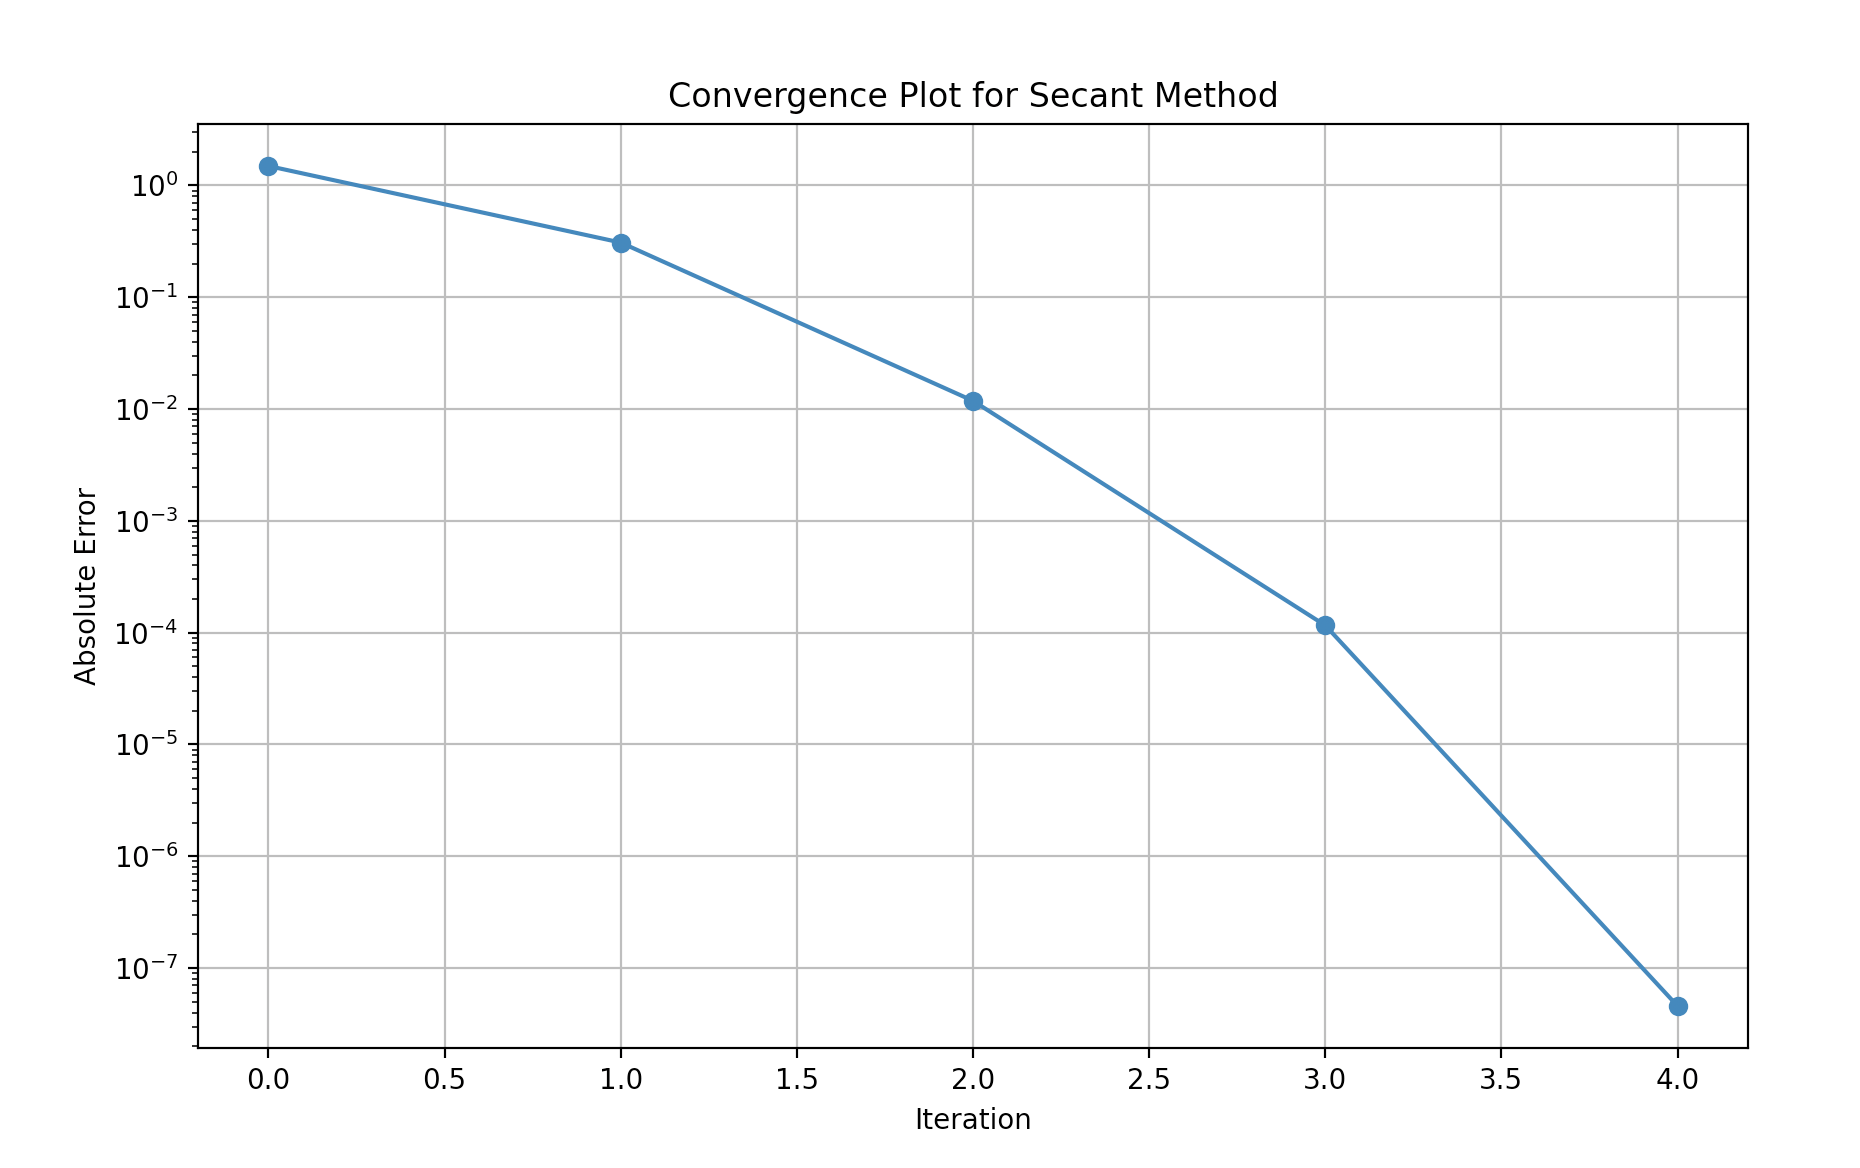
\includegraphics[width=0.9\linewidth]{plot.png}
\\
We can see that the $y$-values (absolute error) decrease with each iteration.
The rate of decrease is faster than a linear decrease (straight line on a log-linear plot) but slower than a quadratic decrease (concave down curve on a log-linear plot).
Given these characteristics, we can confirm that the Secant method converges super-linearly for this problem.

\end{document}
\endinput
%%
%% End of file `sample-authordraft.tex'.
